\chapter{Transmissão dos dados em série}\label{chap:chap4}

Este capítulo aborda o trabalho realizado na segunda parte do projeto, tal como definido em ~\ref{sec:descrição_objetivos}. Esta parte do projeto consiste em transmitir em paralelo para o transmissor GTX existente na FPGA VC7203 que ,através da sua arquitetura, serializa os dados e envia-os através de um cabo físico. Esse mesmo cabo conectado ao recetor GTX irá deserializar para que sejam convertidos novamente para dados em paralelo.

Este processo de serialização e deserialização exige muitos cuidados e aplicações de determinados métodos que permitam manter a integridade do sinal durante a transmissão do mesmo, já como explicado em no capítulo 2 em \ref{serial_theory}. Todavia nesse mesmo capítulo, em \ref{sub:arqGTX} foi já abordado que FPGA VC7203 possui entradas e saídas de alta velocidade com arquiteturas que possuem blocos que permitem a implementação destes mecanismos. Na imagem \ref{fig:gtx_geral_arq} da página \pageref{fig:gtx_geral_arq} visualiza-se uma arquitetura geral dos transcetores, mas estes serão descritos com mais detalhe neste capítulo.

Este capítulo começa por abordar as arquiteturas transmissora e recetora com mais detalhe e quais as características que são vantajosas a este projeto. De seguida serão contempladas as arquiteturas desenvolvidas e explicadas todas as decisões no seu desenvolvimento.

\section{Transmissor} \label{sec:tx_gtx}

Na figura \ref{fig:gtx_tx_arq} da página \pageref{fig:gtx_tx_arq} visualiza-se a arquitetura do transmissor GTX. Assim como já foi mencionado, esta arquitetura possui muitos blocos com diferentes funções que permitem manter a integridade do sinal durante uma transmissão, pelo menos, daquilo que se pode fazer do lado do transmissor.
\begin{figure}[h!]
	\begin{center}
		\leavevmode
		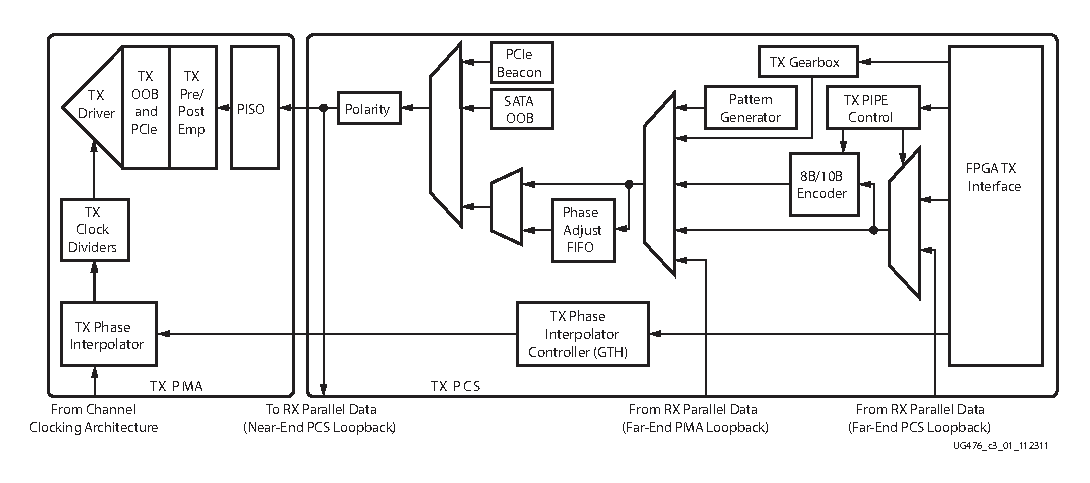
\includegraphics[width=1.0\textwidth]{tx_gtx_arq}
		\caption{Arquitetura do transmissor GTX, retirada de \cite{R011}}
		\label{fig:gtx_tx_arq}
	\end{center}
\end{figure}

Os blocos mais relevantes para o funcionamento do projeto passam de seguida a ser descritos nas próxima subsecções para que se possa entender mais facilmente as arquiteturas desenvolvidas quando estas forem apresentadas.

\subsection{Interface com a FPGA}

Este bloco com o nome de "\textit{FPGA TX Interface}" na arquitetura do transmissor.

\subsection{Codificador 8B/10B}

\subsection{Gerador de padrões pseudo-aleatórios}

\subsection{\textit{Driver} do Transmissor}

\subsection{Interface com a camada física}

\section{Recetor} \label{sec_rx_gtx}

\begin{figure}[h!]
	\begin{center}
		\leavevmode
		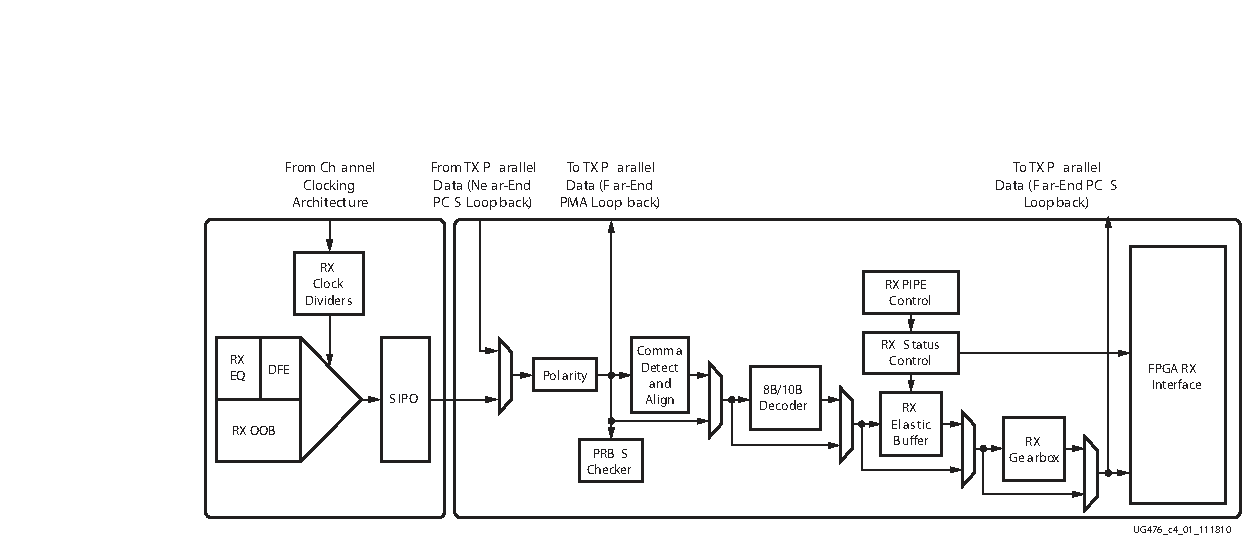
\includegraphics[width=1.0\textwidth]{rx_gtx_arq}
		\caption{Arquitetura do recetor GTX, retirada de \cite{R011}}
		\label{fig:gtx_rx_arq}
	\end{center}
\end{figure}	
	
	
	
	
	
	
	
	
	
	
	
	
	
	
	
	
	%Em \cite{R031} é sugerido que o valor do sinal de relogio de referencia seja o mesmo proveninete da fonte HDMI isto porque a frequência o sinal de relógio de referência deve ser exatamente igual (ou multiplo) da cadência dos dados de entrada.